\documentclass[a4paper]{article}
\usepackage{geometry}
\geometry{a4paper, portrait, margin=0.7in}
\usepackage[english]{babel}
\usepackage[utf8]{inputenc}
\usepackage{amsmath}
\usepackage{enumitem}
\usepackage{graphicx}
\usepackage[colorinlistoftodos]{todonotes}

\title{COL341: Machine Learning \\ \Large{Assignment 1 Report}}

\author{Utkarsh N. Singh, 2015ME10686}

\date{\today}

\begin{document}
\maketitle

\textbf{Note}: For all plots, y-axis is the log-likelihood value.

\section*{Part a. - Full Batch Gradient Descent}
\label{sec:parta}
\subsection*{Constant Learning Rate}
For learning rate = 0.0000001, 500 iterations the log-likelihood plot looks as follows:
\begin{figure}[h!]
\centering
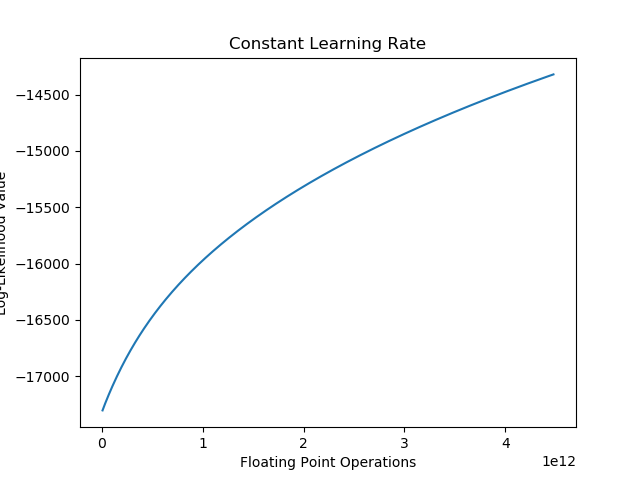
\includegraphics[width=8cm,height=6cm]{clr_0000001_500_7418.png}
\end{figure}

\noindent with model accuracy of \textbf{74.18\%}.
\vskip 0.1in
\noindent For learning rate = 0.0000005, 500 iterations the log-likelihood plot looks as follows:

\begin{figure}[h!]
\centering
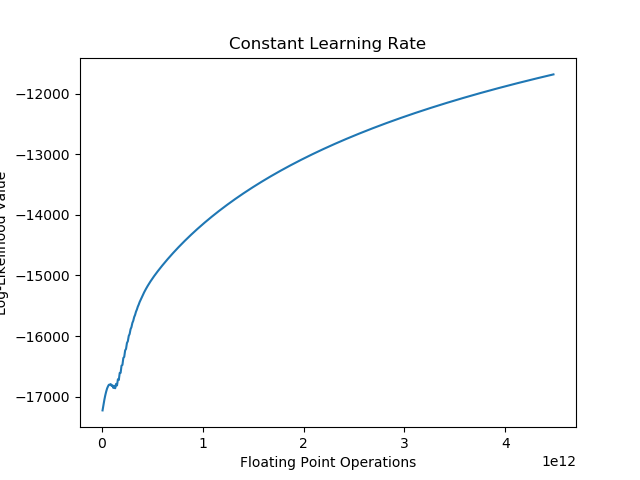
\includegraphics[width=8cm,height=6cm]{clr_0000005_500_8078.png}
\end{figure}

\noindent with model accuracy of \textbf{80.78\%}.
\vskip 0.1in
\noindent Since we learn on a constant rate, it's important to set a value that isn't too large to prevent overshoot. It can be seen that values small overshooting has already began at a rate as small as 0.0000005.

\break
\subsection*{Adaptive Learning Rate}
For learning rate = 0.000001, 500 iterations the log-likelihood plot looks as follows:
\begin{figure}[h!]
\centering
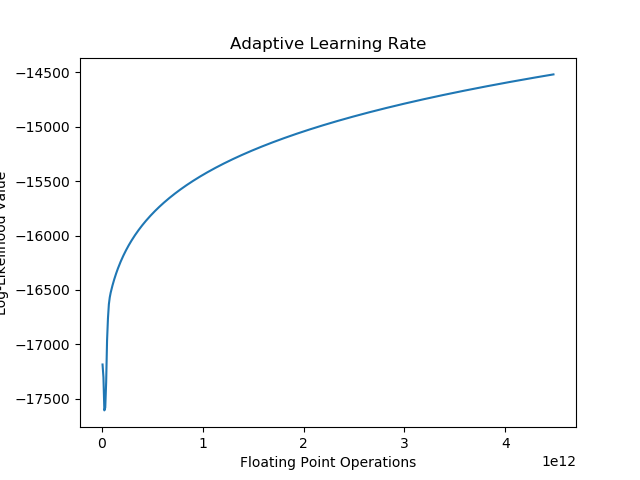
\includegraphics[width=8cm,height=6cm]{adlr_000001_500_65376.png}
\end{figure}

\noindent with model accuracy of \textbf{65.376\%}.
\vskip 0.1in
\noindent For learning rate = 0.00001, 500 iterations the log-likelihood plot looks as follows:

\begin{figure}[h!]
\centering
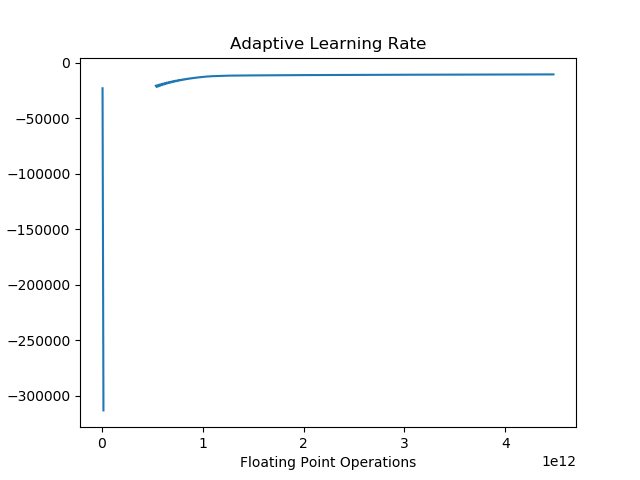
\includegraphics[width=8cm,height=6cm]{adlr_00001_500_82192.png}
\end{figure}

\noindent with model accuracy of \textbf{82.912\%}. (Some values were becoming 'nan' because of the nature of the sigmoid function)
\vskip 0.1in
\noindent Here as the learning rate decreases with time, it's better to start with a much larger value, and it helps reach the optimum faster without overshooting.

\subsection*{Exact Line Search}
For learning rate = 0.000001, 100 iterations the log-likelihood plot looks as follows:

\begin{figure}[h!]
\centering
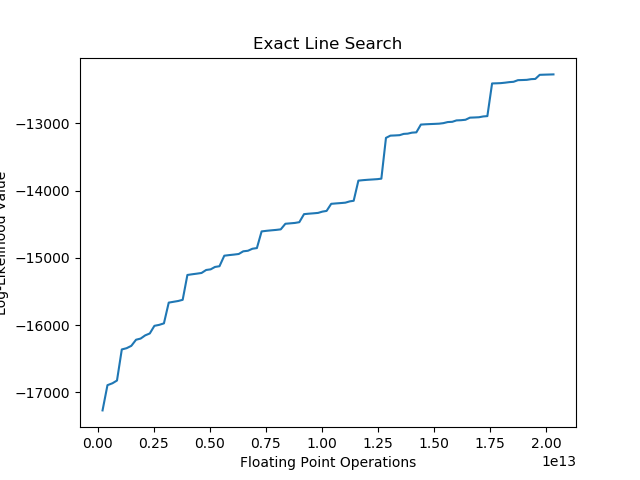
\includegraphics[width=8cm,height=6cm]{els_000001_100_79628.png}
\end{figure}

\noindent with model accuracy of \textbf{79.628\%}.
\vskip 0.1in
\noindent For learning rate = 0.000005, 100 iterations the log-likelihood plot looks as follows:

\begin{figure}[h!]
\centering
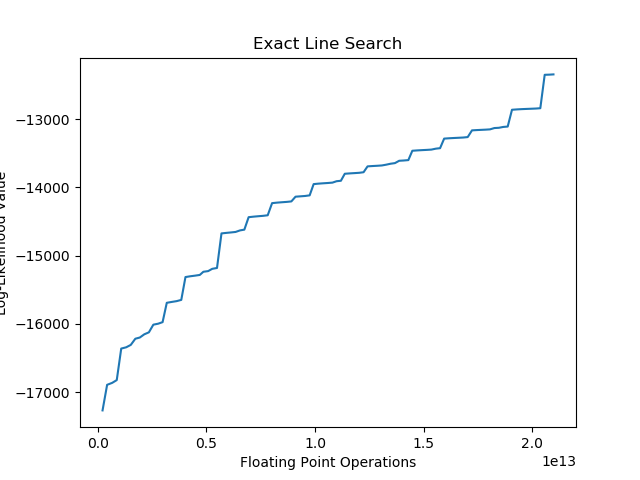
\includegraphics[width=8cm,height=6cm]{els_000005_100_7934.png}
\end{figure}

\noindent with model accuracy of \textbf{79.34\%}. 
\vskip 0.1in
\noindent Since Exact Search searches for the optimum value of learning rate before making a gradient descent step, there isn't much difference in the log-probability value, and thus the accuracy.

\section*{Part b. - Stochastic Gradient Descent}
\label{sec:partb}
\subsection*{Constant Learning Rate}
For learning rate = 0.00005, 500 iterations the log-likelihood plot looks as follows:
\begin{figure}[h!]
\centering
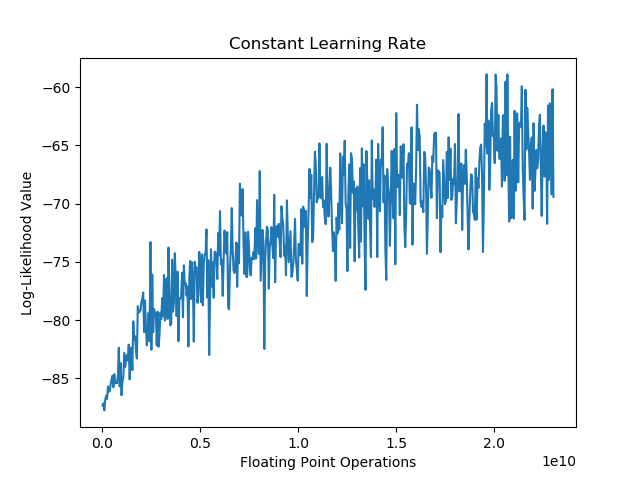
\includegraphics[width=8cm,height=6cm]{b_clr_00005_500_76472.png}
\end{figure}

\noindent with model accuracy of \textbf{76.472\%}.
\vskip 0.1in
\noindent For learning rate = 0.0001, 500 iterations the log-likelihood plot looks as follows:

\begin{figure}[h!]
\centering
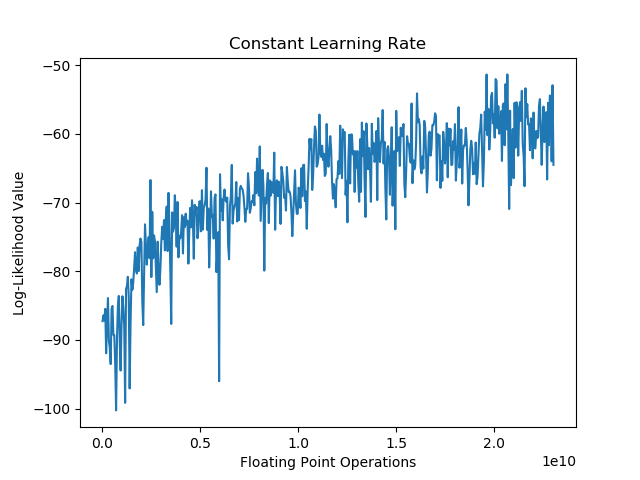
\includegraphics[width=8cm,height=6cm]{b_clr_0001_500_7418.png}
\end{figure}

\noindent with model accuracy of \textbf{74.18\%}.
\vskip 0.1in
\noindent Plot is noisy because at every step we look at a 'new' batch of data, one which we didn't process in the previous step. This affects the direction of gradient, and thus the steps we make towards reaching the optimum. It is relatively difficult to determine now that which learning rate value would be a good one. 

\subsection*{Adaptive Learning Rate}
For learning rate = 0.0001, 500 iterations the log-likelihood plot looks as follows:
\begin{figure}[h!]
\centering
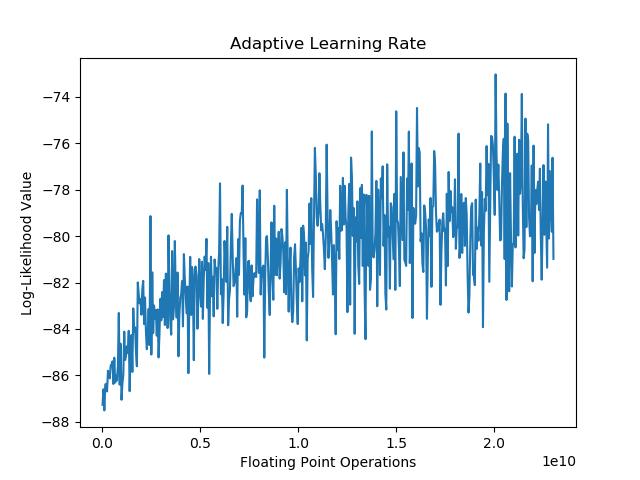
\includegraphics[width=8cm,height=6cm]{b_adlr_0001_500_7006.png}
\end{figure}

\noindent with model accuracy of \textbf{70.06\%}.
\vskip 0.1in
\noindent For learning rate = 0.001, 500 iterations the log-likelihood plot looks as follows:

\begin{figure}[h!]
\centering
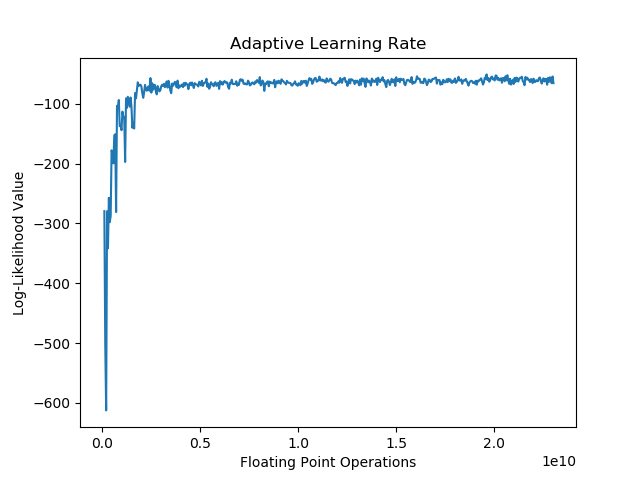
\includegraphics[width=8cm,height=6cm]{b_adlr_001_500_79024.png}
\end{figure}

\noindent with model accuracy of \textbf{79.024\%}.

\subsection*{Exact Line Search}
For learning rate = 0.000001, 500 iterations the log-likelihood plot looks as follows:

\begin{figure}[h!]
\centering
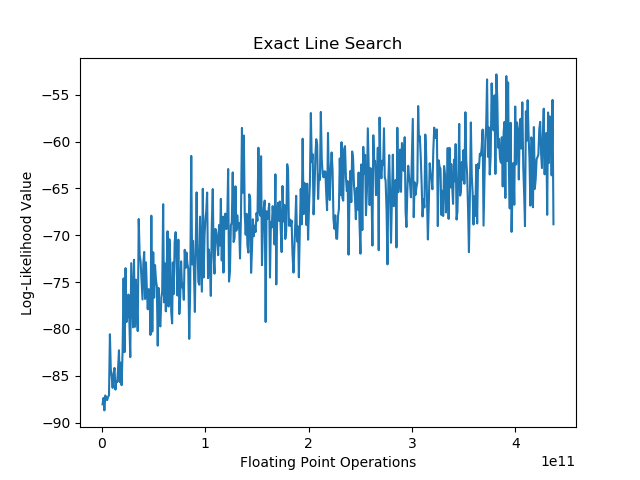
\includegraphics[width=8cm,height=5.3cm]{b_els_000001_500_7994.png}
\end{figure}

\noindent with model accuracy of \textbf{79.94\%}.
\vskip 0.1in
\noindent For learning rate = 0.000005, 500 iterations the log-likelihood plot looks as follows:


\begin{figure}[h!]
\centering
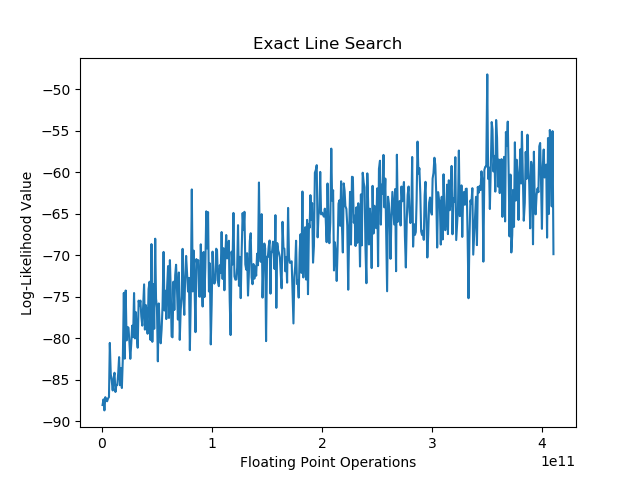
\includegraphics[width=8cm,height=6cm]{b_els_000005_500_79464.png}
\end{figure}

\noindent with model accuracy of \textbf{79.464\%}.

\section*{Part c. - Stopping Criterion}
\label{sec:partc}

We will experiment with two stopping criteria, on adaptive learning rate.

\begin{enumerate}
	\item Change in norm of gradient of log-probability
    \item Change in log-probability value
\end{enumerate}

\vskip 0.15in
\noindent We will fix an initial learning rate, and do a full batch gradient descent.

\subsection*{Change in norm of gradient of log-probability}
For the above stopping criteria with initial learning rate of 0.00003, the gradient descent ran for 11493 iterations until finally converging on the predefined condition that the change in norm of gradient isn't more than 0.01. The log-likelihood plot looks as follows:
\begin{figure}[h!]
\centering
\includegraphics[width=8cm,height=6cm]{c_norm_0_00003.png}
\end{figure}

\noindent with model accuracy of \textbf{87.636\%}. (Some values were becoming 'nan' because of the nature of the sigmoid function)
\vskip 0.1in

\subsection*{Change in log-probability value}
For the above stopping criteria with initial learning rate of 0.00001, the gradient descent ran for 7939 iterations until finally converging on the predefined condition that the change in norm of gradient isn't more than 0.1. The log-likelihood plot looks as follows:

\break
\begin{figure}[h!]
\centering
\includegraphics[width=8cm,height=6cm]{c_diff_0_00001.png}
\end{figure}

\noindent with model accuracy of \textbf{85.844\%}. (Some values were becoming 'nan' because of the nature of the sigmoid function)
\vskip 0.1in

\subsection*{Conclusions}
It can be seen clearly that among the three strategies of learning, \textbf{Adaptive Learning Rate} seem to perform the best in terms of accuracy and lop-probability likelihood value, however there may be few overshoots observed that might sometimes hamper the learning. In that regards, \textbf{Exact Line Search} seems to be more robust, because before every step, we ensure to take one that gives us the best result without overshooting. \textbf{Constant Learning Rate} requires us to be very careful with the learning rate value, since too small a value will result in slow convergence, but a high value will never take us the optimum.

\end{document}
